%%%%%%%%%%%%%%%%%%%%%%%%%%%%%%%%%%%%%%%%%%%%%%%%%%%%%%%%%%%%%%%%
%
%  Template for homework of Introduction to Machine Learning.
%
%  Fill in your name, lecture number, lecture date and body
%  of homework as indicated below.
%
%%%%%%%%%%%%%%%%%%%%%%%%%%%%%%%%%%%%%%%%%%%%%%%%%%%%%%%%%%%%%%%%


\documentclass[11pt,letter,notitlepage]{article}
%Mise en page
\usepackage[left=2cm, right=2cm, lines=45, top=0.8in, bottom=0.7in]{geometry}
\usepackage{fancyhdr}
\usepackage{fancybox}
\usepackage{graphicx}
\usepackage{pdfpages} 
\usepackage{enumitem}
\usepackage{ctex}
\renewcommand{\headrulewidth}{1.5pt}
\renewcommand{\footrulewidth}{1.5pt}
\pagestyle{fancy}
\newcommand\Loadedframemethod{TikZ}
\usepackage[framemethod=\Loadedframemethod]{mdframed}

\usepackage{amssymb,amsmath}
\usepackage{amsthm}
\usepackage{thmtools}

\setlength{\topmargin}{0pt}
\setlength{\textheight}{9in}
\setlength{\headheight}{0pt}

\setlength{\oddsidemargin}{0.25in}
\setlength{\textwidth}{6in}

%%%%%%%%%%%%%%%%%%%%%%%%
%% Define the Exercise environment %%
%%%%%%%%%%%%%%%%%%%%%%%%
\mdtheorem[
topline=false,
rightline=false,
leftline=false,
bottomline=false,
leftmargin=-10,
rightmargin=-10
]{exercise}{\textbf{Exercise}}
%%%%%%%%%%%%%%%%%%%%%%%
%% End of the Exercise environment %%
%%%%%%%%%%%%%%%%%%%%%%%

%%%%%%%%%%%%%%%%%%%%%%%
%% Define the Solution Environment %%
%%%%%%%%%%%%%%%%%%%%%%%
\declaretheoremstyle
[
spaceabove=0pt, 
spacebelow=0pt, 
headfont=\normalfont\bfseries,
notefont=\mdseries, 
notebraces={(}{)}, 
headpunct={:\quad}, 
headindent={},
postheadspace={ }, 
postheadspace=4pt, 
bodyfont=\normalfont, 
qed=$\blacksquare$,
preheadhook={\begin{mdframed}[style=myframedstyle]},
	postfoothook=\end{mdframed},
]{mystyle}

\declaretheorem[style=mystyle,title=Solution,numbered=no]{solution}
\mdfdefinestyle{myframedstyle}{%
	topline=false,
	rightline=false,
	leftline=false,
	bottomline=false,
	skipabove=-6ex,
	leftmargin=-10,
	rightmargin=-10}
%%%%%%%%%%%%%%%%%%%%%%%
%% End of the Solution environment %%
%%%%%%%%%%%%%%%%%%%%%%%

%% Homework info.
\newcommand{\posted}{\text{Seq. 20, 2019}}       			%%% FILL IN POST DATE HERE
\newcommand{\due}{\text{Seq. 30, 2019}} 			%%% FILL IN Due DATE HERE
\newcommand{\hwno}{\text{1}} 		           			%%% FILL IN LECTURE NUMBER HERE


%%%%%%%%%%%%%%%%%%%%
%% Put your information here %%
%%%%%%%%%%%%%%%%%%%
\newcommand{\name}{\text{Jiahuan Yu}}  	          			%%% FILL IN YOUR NAME HERE
\newcommand{\id}{\text{PB17121687}}		       			%%% FILL IN YOUR ID HERE
%%%%%%%%%%%%%%%%%%%%
%% End of the student's info %%
%%%%%%%%%%%%%%%%%%%


\newcommand{\proj}[2]{\textbf{P}_{#2} (#1)}
\newcommand{\lspan}[1]{\textbf{span}  (#1)  }
\newcommand{\rank}[1]{ \textbf{rank}  (#1)  }
\newcommand{\dom}{ \textbf{dom}  }
\newcommand{\RNum}[1]{\uppercase\expandafter{\romannumeral #1\relax}}


\lhead{
	\textbf{\name}
}
\rhead{
	\textbf{\id}
}
\chead{\textbf{
		Homework \hwno
}}


\begin{document}
\vspace*{-4\baselineskip}
\thispagestyle{empty}


\begin{center}
	{\bf\large Introduction to Machine Learning}\\
	{Fall 2019}\\
	University of Science and Technology of China
\end{center}

\noindent
Lecturer: Jie Wang  			 %%% FILL IN LECTURER HERE
\hfill
Homework \hwno
\\
Posted: \posted
\hfill
Due: \due
\\
Name: \name
\hfill
ID: \id
\hfill

\noindent
\rule{\textwidth}{2pt}

\medskip





%%%%%%%%%%%%%%%%%%%%%%%%%%%%%%%%%%%%%%%%%%%%%%%%%%%%%%%%%%%%%%%%
%% BODY OF HOMEWORK GOES HERE
%%%%%%%%%%%%%%%%%%%%%%%%%%%%%%%%%%%%%%%%%%%%%%%%%%%%%%%%%%%%%%%%

\textbf{Notice, }to get the full credits, please present your solutions step by step.

\begin{exercise}[Linear regression \textnormal{20pts}]
	Given a data set $\{ (x_i ,y_i) \}_{i=1}^{n}$, where $x_i,y_i\in \mathbb{R}$.
	\begin{enumerate}
		\item If we want to fit the data by a linear model
		      \begin{align}\label{eqn:linear}
			      y =  w_0 + w_1 x,
		      \end{align}
		      please find $\hat{w}_0$ and $\hat{w}_1$ by the least squares approach (you need to find expressions of $\hat{w}_0$ and $\hat{w}_1$ by $\{ (x_i ,y_i) \}_{i=1}^{n}$, respectively).
		\item \textbf{Programming Exercise} We provide you a data set $\{ (x_i ,y_i) \}_{i=1}^{30}$. Consider the model in (\ref{eqn:linear}) and the one as follows:
		      \begin{align}\label{eqn:linear-quadratic}
			      y =  w_0 + w_1 x+ w_2 x^2.
		      \end{align}
		      Which model do you think fits better the data? Please detail your approach first and then implement it by your favorite programming language. The required output includes
		      \begin{enumerate}
			      \item your detailed approach step by step;
			      \item your code with detailed comments according to your planned approach;
			      \item a plot showing the data and the fitting models;
			      \item the model you finally choose [$\hat{w}_0$ and $\hat{w}_1$ if you choose the model in (\ref{eqn:linear}), or $\hat{w}_0$, $\hat{w}_1$, and $\hat{w}_2$ if you choose the model in (\ref{eqn:linear})].
		      \end{enumerate}
	\end{enumerate}

\end{exercise}

\begin{solution}
	\begin{enumerate}
		\item 定义
		      $$S(f(i))=\sum_{i=1}^{n}{f(i)}$$
		      其中 $f(i)$ 为任意关于 $i$ 的表达式。令
		      $$\hat{y_i} = \hat{w}_0+\hat{w}_1 x_i$$
		      $$\varepsilon = S^2(\hat{y}_i-y_i)
			      = S^2(\hat{w}_0+\hat{w}_1 x_i-y_i)$$
		      最小二乘法要求
		      $$\arg\min_{\hat{w}_0,\hat{w}_1} \varepsilon$$
		      则
		      $$\begin{aligned}
				      \frac{\partial\varepsilon}{\partial \hat{w}_0}
				       & = 2 S(\hat{w}_0+\hat{w}_1 x_i-y_i)           \\
				       & = 2n\hat{w}_0 + 2\hat{w}_1 S(x_i) - 2 S(y_i)
			      \end{aligned}$$
		      $$\begin{aligned}
				      \frac{\partial\varepsilon}{\partial \hat{w}_1}
				       & = 2 S((\hat{w}_0+\hat{w}_1 x_i-y_i)x_i)                   \\
				       & = 2\hat{w}_0 S(x_i) + 2 \hat{w}_1 S(x_i^2) - 2 S(x_i y_i)
			      \end{aligned}$$
		      令
		      $$\frac{\partial\varepsilon}{\partial \hat{w}_0} = \frac{\partial\varepsilon}{\partial \hat{w}_1} = 0$$
		      解得
		      $$\begin{aligned}
				      \hat{w}_0 & = \frac
				      {S({x_i}^2) S(y_i) - S(x_i) S(x_i y_i)}
				      {n S({x_i}^2) - S^2(x_i)} \\
				      \hat{w}_1 & = \frac
				      {n S(x_i y_i) - S(x_i) S(y_i)}
				      {n S({x_i}^2) - S^2(x_i)}
			      \end{aligned}$$

		\item 如上题,在线性回归中,求解回归系数的方程组为
		      \begin{align}\label{linear-solution-equation}
			      \begin{bmatrix}
				      n      & S(x_i)   \\
				      S(x_i) & S(x_i^2)
			      \end{bmatrix}
			      \begin{bmatrix}
				      \hat{w}_0 \\ \hat{w}_1
			      \end{bmatrix}
			      = \begin{bmatrix}
				      S(y_i) \\ S(x_i y_i)
			      \end{bmatrix}
		      \end{align}
		      在二次回归中
		      $$\varepsilon=S^2(\hat{w}_0+\hat{w}_1 x_i +\hat{w}_2 x_i^2 -y_i)$$
		      令
		      $$\frac{\partial\varepsilon}{\partial\hat{w}_0}
			      =\frac{\partial\varepsilon}{\partial\hat{w}_1}
			      =\frac{\partial\varepsilon}{\partial\hat{w}_2}=0$$
		      整理可得求解回归系数的方程组
		      \begin{align}\label{quadratic-solution-equation}
			      \begin{bmatrix}
				      n        & S(x_i)   & S(x_i^2) \\
				      S(x_i)   & S(x_i^2) & S(x_i^3) \\
				      S(x_i^2) & S(x_i^3) & S(x_i^4)
			      \end{bmatrix}
			      \begin{bmatrix}
				      \hat{w}_0 \\ \hat{w}_1 \\ \hat{w}_2
			      \end{bmatrix}
			      =\begin{bmatrix}
				      S(y_i) \\ S(x_i y_i) \\ S(x_i^2 y_i)
			      \end{bmatrix}
		      \end{align}
		      求解 (\ref{linear-solution-equation}) 和 (\ref{quadratic-solution-equation}) 即可获得回归系数,分别计算线性回归和二次回归情况下的 $\varepsilon$, 较小的那个模型拟合更优。

		      以上求解过程的程序实现见 solution1.2.py, 输出的图片见 plot.png, 如下:

		      \begin{center}
			      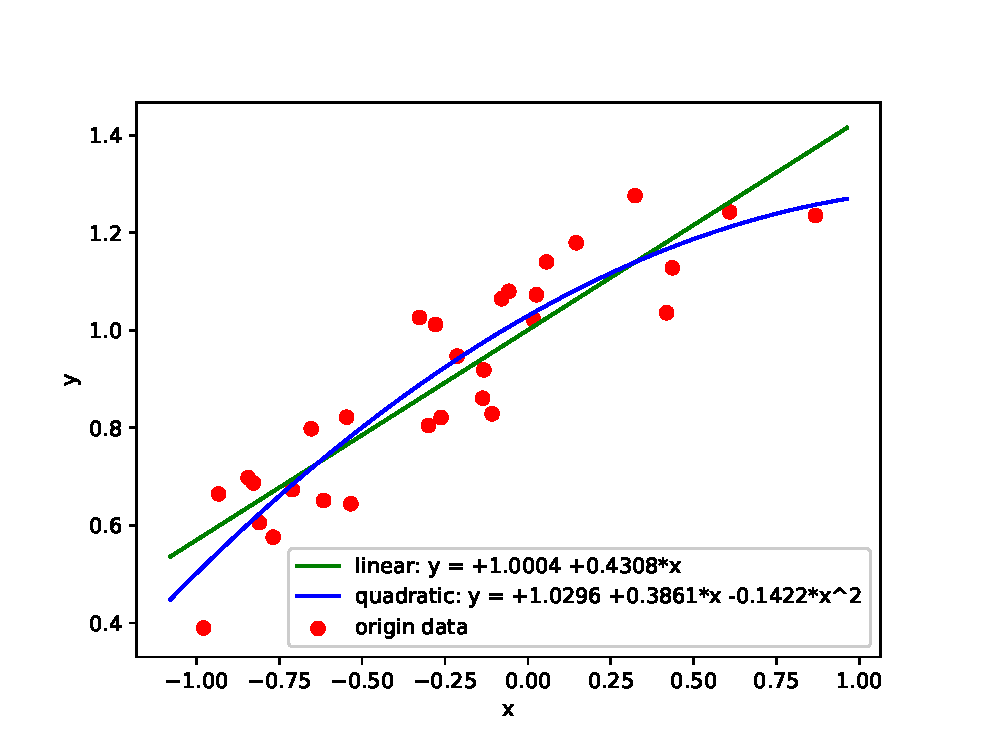
\includegraphics[width=0.8\textwidth]{plot1.2.eps}
		      \end{center}

	\end{enumerate}
\end{solution}
\newpage

\begin{exercise}[Rank of matrices \textnormal{20pts}]
	Let $\mathbf{A} \in \mathbb{R}^{m\times n}$ and $\mathbf{B}\in \mathbb{R}^{n\times p}$.
	\begin{enumerate}
		\item Please show that
		      \begin{enumerate}
			      \item $\rank{\mathbf{A}} = \rank{\mathbf{A}^{\top}}$;
			      \item $\rank{\mathbf{A}\mathbf{B}} \leq \rank{\mathbf{A}}$;
			      \item $\rank{\mathbf{A}\mathbf{B}} \leq \rank{\mathbf{B}}$;
			      \item $\rank{\mathbf{A}} = \rank{\mathbf{A}^{\top}  \mathbf{A}}$.
		      \end{enumerate}
		\item The \emph{column space} of $\mathbf{A}$ is defined by
		      \begin{align*}
			      \mathcal{C}(\mathbf{A} ) = \{ \mathbf{y}\in \mathbb{R}^m : \mathbf{y} = \mathbf{Ax},\,\mathbf{x}\in\mathbb{R}^n\}.
		      \end{align*}
		      The \emph{null space} of $\mathbf{A}$ is defined by
		      \begin{align*}
			      \mathcal{N}(\mathbf{A})  = \{ \mathbf{x}\in \mathbb{R}^n : \mathbf{Ax}=0\}.
		      \end{align*}
		      Notice that, the rank of $\mathbf{A}$ is the dimension of the column space of $\mathbf{A}$.

		      Please show that:
		      \begin{enumerate}
			      \item $\rank{\mathbf{A}} + \dim ( \mathcal{N}( \mathbf{A} ) ) = n$;
			      \item let $\mathbf{y}\in \mathbb{R}^m$, show that $\mathbf{y}=0$ if and only if $\mathbf{a}_i^{\top}\mathbf{y}=0$ for $i=1,\ldots,m$, where $\{\mathbf{a}_1,\mathbf{a}_2,\ldots,\mathbf{a}_m\}$ is a basis of $\mathbb{R}^m$.
		      \end{enumerate}
	\end{enumerate}
\end{exercise}

\begin{solution}
	\begin{enumerate}
		\item \begin{enumerate}
			      \item 设
			            $$\mathbf{A}=\mathbf{P}\mathbf{A_1}\mathbf{Q},
				            \mathbf{A_1}=\begin{pmatrix}
					            \mathbf{I_r} & \mathbf{O} \\
					            \mathbf{O}   & \mathbf{O} \\
				            \end{pmatrix}$$
			            其中 $\mathbf{I_r}$ 是 $r$ 阶单位矩阵,$P$, $Q$ 是可逆矩阵。有
			            $$\rank{\mathbf{A}}=\rank{\mathbf{A_1}}=r$$
			            所以
			            $$\rank{\mathbf{A}^{\top}}
				            =\rank{\mathbf{Q}^{\top}\mathbf{A_1}^{\top}\mathbf{P}^{\top}}
				            =\rank{\mathbf{A_1}^{\top}}
				            =\rank{\mathbf{A_1}}
				            =\rank{A}$$
			      \item 设
			            $$\mathbf{A}=\mathbf{P_1}\mathbf{A_1}\mathbf{Q_1}, \mathbf{B}=\mathbf{P_2}\mathbf{B_1}\mathbf{Q_2}$$
			            $$\mathbf{A_1}=\begin{pmatrix}
					            \mathbf{I_r} & \mathbf{O} \\
					            \mathbf{O}   & \mathbf{O} \\
				            \end{pmatrix},
				            \mathbf{B_1}=\begin{pmatrix}
					            \mathbf{I_s} & \mathbf{O} \\
					            \mathbf{O}   & \mathbf{O} \\
				            \end{pmatrix}$$
			            其中 $\mathbf{P_1}$, $\mathbf{P_2}$, $\mathbf{Q_1}$, $\mathbf{Q_2}$ 是可逆矩阵。

			            令 $\mathbf{Q}=\mathbf{Q_1}\mathbf{P_2}$ 则有
			            $$\mathbf{A}\mathbf{B}
				            =\mathbf{P_1}\mathbf{A_1}\mathbf{Q_1}\mathbf{P_2}\mathbf{B_1}\mathbf{Q_2}
				            =\mathbf{P_1} \left(\mathbf{A_1}\mathbf{R}\mathbf{B_1}\right) \mathbf{Q_2}$$
			            $$\mathbf{A_1}\mathbf{R}\mathbf{B_1}
				            =\begin{pmatrix}
					            \mathbf{I_r} & \mathbf{O} \\
					            \mathbf{O}   & \mathbf{O} \\
				            \end{pmatrix}
				            \begin{pmatrix}
					            \mathbf{R_1} & \mathbf{R_2} \\
					            \mathbf{R_3} & \mathbf{R_4} \\
				            \end{pmatrix}
				            \begin{pmatrix}
					            \mathbf{I_s} & \mathbf{O} \\
					            \mathbf{O}   & \mathbf{O} \\
				            \end{pmatrix}
				            =\begin{pmatrix}
					            \mathbf{R_1} & \mathbf{O} \\
					            \mathbf{O}   & \mathbf{O} \\
				            \end{pmatrix}$$
			            其中 $\mathbf{R_1} \in \mathbb{R}^{r\times s}$. 而
			            $$\rank{\mathbf{R_1}} \le \min \left\{r, s\right\}$$
			            所以
			            $$\begin{aligned}
					            \rank{\mathbf{A}\mathbf{B}}
					             & = \rank{\mathbf{P_1}
						            \begin{pmatrix}
							            \mathbf{R_1} & \mathbf{O} \\
							            \mathbf{O}   & \mathbf{O} \\
						            \end{pmatrix}
						            \mathbf{Q_2}}                                                   \\
					             & = \rank{\begin{pmatrix}
							            \mathbf{R_1} & \mathbf{O} \\
							            \mathbf{O}   & \mathbf{O} \\
						            \end{pmatrix}}                          \\
					             & \le \min \left\{\rank{\mathbf{A}}, \rank{\mathbf{B}}\right\}
				            \end{aligned}$$
			            所以
			            $$\rank{\mathbf{A}\mathbf{B}} \le \rank{\mathbf{A}}$$
			      \item 由上一小问
			            $$\rank{\mathbf{A}\mathbf{B}} \le \min \left\{\rank{\mathbf{A}}, \rank{\mathbf{B}}\right\}$$
			            可得
			            $$\rank{\mathbf{A}\mathbf{B}} \le \rank{\mathbf{B}}$$
			      \item 设
			            $$\mathbf{A}=\mathbf{P}\mathbf{A_1}\mathbf{Q},
				            \mathbf{A_1}=\begin{pmatrix}
					            \mathbf{I_r} & \mathbf{O} \\
					            \mathbf{O}   & \mathbf{O} \\
				            \end{pmatrix}$$
			            其中 $\mathbf{I_r}$ 是 $r$ 阶单位矩阵,$P$, $Q$ 是可逆矩阵。

			            设 $\mathbf{R}=\mathbf{P}^{\top}\mathbf{P}$,
			            $\mathbf{R_r}\in\mathbb{R}^{r\times r}$ 且
			            $$\mathbf{R}=\begin{pmatrix}
					            \mathbf{R_r} & \mathbf{R_1} \\
					            \mathbf{R_2} & \mathbf{R_3}
				            \end{pmatrix}$$
			            因此
			            $$\begin{aligned}
					            \rank{\mathbf{A}^{\top}\mathbf{A}}
					             & = \rank{\mathbf{Q}^{\top}\mathbf{A_1}^{\top}\mathbf{P}^{\top}\mathbf{P}\mathbf{A_1}\mathbf{Q}} \\
					             & = \rank{\mathbf{Q}^{\top}
						            \begin{pmatrix}
							            \mathbf{I_r} & \mathbf{O} \\
							            \mathbf{O}   & \mathbf{O} \\
						            \end{pmatrix}
						            \mathbf{R}
						            \begin{pmatrix}
							            \mathbf{I_r} & \mathbf{O} \\
							            \mathbf{O}   & \mathbf{O} \\
						            \end{pmatrix}
						            \mathbf{Q}}                                                                                       \\
					             & = \rank{\mathbf{Q}^{\top}
						            \begin{pmatrix}
							            \mathbf{R_r} & \mathbf{O} \\
							            \mathbf{O}   & \mathbf{O} \\
						            \end{pmatrix}
						            \mathbf{Q}}                                                                                       \\
					             & = \rank{
						            \begin{pmatrix}
							            \mathbf{R_r} & \mathbf{O} \\
							            \mathbf{O}   & \mathbf{O} \\
						            \end{pmatrix}}
				            \end{aligned}$$
			            由于 $\rank{R}$ 是满秩的,其子阵 $\mathbf{R_r}$ 也是满秩的,因此
			            $$
				            \rank{\mathbf{A}^{\top}\mathbf{A}}
				            = \rank{
					            \begin{pmatrix}
						            \mathbf{R_r} & \mathbf{O} \\
						            \mathbf{O}   & \mathbf{O} \\
					            \end{pmatrix}}
				            = \rank{\mathbf{R_r}}
				            = r
				            = \rank{\mathbf{A}}
			            $$
		      \end{enumerate}
		\item \begin{enumerate}
			      \item 因为 $\rank{\mathbf{A}}=r$, 所以 $\mathbf{A}$ 可以通过初等行变换变为以下形式
			            $$\mathbf{J}=\begin{pmatrix}
					            c_{11} & \cdots & c_{1,j_2 -1} & \cdots    & \cdots & \cdots       & \cdots    & \cdots & c_{1n} \\
					            0      & \cdots & 0            & c_{2,j_2} & \cdots & c_{2,j_3 -1} & \cdots    & \cdots & c_{2n} \\
					            0      & \cdots & \cdots       & 0         & \cdots & 0            & c_{3,j_3} & \cdots & c_{3n} \\
					            \vdots &        &              & \vdots    &        & \vdots       & \vdots    & \ddots & \vdots \\
					            0      & \cdots & \cdots       & 0         & \cdots & 0            & 0         & \cdots & c_{rn} \\
					            0      & \cdots & \cdots       & \cdots    & \cdots & \cdots       & \cdots    & \cdots & 0      \\
					            \vdots &        &              &           &        &              &           &        & \vdots \\
					            0      & \cdots & \cdots       & \cdots    & \cdots & \cdots       & \cdots    & \cdots & 0
				            \end{pmatrix}$$
			            所以 $\mathbf{Ax}=0$ 等价于 $\mathbf{Jx}=0$.

			            记 $\mathbf{x}$ 中除了 $x_{j_1}, x_{j_2}, \cdots, x_{j_r} (j_1=1)$ 以外的分量为 $t_1, t_2, \cdots, t_{n-r}$

			            当 $t_1, t_2, \cdots, t_{n-r}$ 确定后,剩下的分量组成线性方程组
			            $$\begin{pmatrix}
					            c_{1 j_1} & c_{1 j_2} & \cdots & c_{1 j_r} \\
					            0         & c_{2 j_2} & \cdots & c_{2 j_r} \\
					            \vdots    & \vdots    & \ddots & \vdots    \\
					            0         & 0         & \cdots & c_{r j_r}
				            \end{pmatrix}
				            \begin{pmatrix}
					            x_{j_1} \\ x_{j_2}\\ \vdots\\ x_{j_r}
				            \end{pmatrix}=0$$
			            可继续化为
			            $$\begin{pmatrix}
					            d_{11} & 0      & \cdots & 0      \\
					            0      & d_{22} & \cdots & 0      \\
					            \vdots & \vdots & \ddots & \vdots \\
					            0      & 0      & \cdots & d_{rr}
				            \end{pmatrix}
				            \begin{pmatrix}
					            x_{j_1} \\ x_{j_2}\\ \vdots\\ x_{j_r}
				            \end{pmatrix}=0$$
			            此方程组有唯一解 $x_{j_1}=x_{j_2}=\cdots=x_{j_r}=0$.

			            因此 $\mathbf{Ax}=0$ 的解可以写成

			            $$\begin{pmatrix}
					            x_1 \\ x_2 \\ \vdots \\ x_n
				            \end{pmatrix}
				            =\begin{pmatrix}
					            h_{11} & h_{12} & \cdots & h_{1,n-r} \\
					            h_{21} & h_{22} & \cdots & h_{2,n-r} \\
					            \vdots & \vdots & \ddots & \vdots    \\
					            h_{n1} & h_{n2} & \cdots & h_{n,n-r}
				            \end{pmatrix}
				            \begin{pmatrix}
					            t_1 \\t_2 \\\vdots\\t_{n-r}
				            \end{pmatrix}
				            =t_1\mathbf{h_1}+t_2\mathbf{h_2}+\cdots+t_{n-r}\mathbf{h_{n-r}}$$
			            其中
			            $$\mathbf{h_i}=\begin{pmatrix}
					            h_{1i} \\h_{2i}\\\vdots\\h_{ni}
				            \end{pmatrix}$$

			            若 $t_1\mathbf{h_1}+t_2\mathbf{h_2}+\cdots+t_{n-r}\mathbf{h_{n-r}}=0$.

			            则 $x_1=x_2=\cdots=x_n=0$.

			            则 $t_1=t_2=\cdots=t_{n-r}=0$.

			            所以 $h_1, h_2, \cdots, h_{n-r}$ 相互独立。

			            所以 $\dim(\mathcal{N}(\mathbf{A})=n-r$.

			            所以 $\rank{\mathbf{A}}+\dim(\mathcal{N}(\mathbf{A}))=n$.
			      \item \begin{enumerate}
				            \item 必要性:证明 $\mathbf{y}=0 \implies \mathbf{a}_i^\top \mathbf{y}=0$

				                  因为 $\mathbf{a}_i^\top \neq 0$, 所以 $\mathbf{y}=0$.

				            \item 充分性:证明 $\mathbf{y}=0 \impliedby \mathbf{a}_i^\top \mathbf{y}=0$

				                  $$(\mathbf{a}_1+\mathbf{a}_2+\cdots+\mathbf{a}_m)\mathbf{y}=0$$

				                  因为 $\left\{\mathbf{a}_1, \mathbf{a}_2,\cdots,\mathbf{a}_m\right\}$ 是基向量, 所以 $\mathbf{a}_1+\mathbf{a}_2+\cdots+\mathbf{a}_m \neq 0$,

				                  否则有 $\mathbf{a}_1=-\mathbf{a}_2-\cdots-\mathbf{a}_m$, 不符合基向量的定义。

				                  所以 $\mathbf{y}=0$

			            \end{enumerate}
		      \end{enumerate}
	\end{enumerate}
\end{solution}
\newpage

\begin{exercise}[Projection \textnormal{30pts}]
	Let $C \subset \mathbb{R}^n$ be a closed convex set and $\mathbf{x} \in \mathbb{R}^n$. Define
	\begin{align*}
		\proj{\mathbf{x}}{C} = \arg\min_{\mathbf{y} \in C}\| \mathbf{y} - \mathbf{x} \|_2.
	\end{align*}
	We call $\proj{\mathbf{x}}{C}$ the projection of the point $\mathbf{x}$ onto the convex set $C$.
	\begin{enumerate}
		\item Show that any finite dimensional space is convex.
		\item Let $\mathbf{v}_i \in \mathbb{R}^n$, $i=1,\ldots,d$ with $d\leq n$, which are linearly independent.
		      \begin{enumerate}
			      \item For any $\mathbf{w}\in \mathbb{R}^n$, please find $\proj{\mathbf{w}}{\mathbf{v}_1}$, which is the projection of $\mathbf{w}$ onto the subspace spanned by $\mathbf{v}_1$.
			      \item Please show $\proj{\cdot}{\mathbf{v}_1}$ is a linear map, i.e.,
			            \begin{align*}
				            \proj{\alpha\mathbf{u}+\beta\mathbf{w}}{\mathbf{v}_1}=\alpha\proj{\mathbf{u}}{\mathbf{v}_1} + \beta \proj{\mathbf{w}}{\mathbf{v}_1},
			            \end{align*}
			            where $\alpha,\beta\in\mathbb{R}$ and $\mathbf{w}\in\mathbb{R}^n$.
			      \item Please find the projection matrix corresponding to the linear map $\proj{\cdot}{\mathbf{v}_1}$, i.e., find the matrix $\mathbf{H}_1\in\mathbb{R}^{n\times n}$ such that
			            \begin{align*}
				            \proj{\mathbf{w}}{\mathbf{v}_1}=\mathbf{H}_1\mathbf{w}.
			            \end{align*}
			      \item Let $\mathbf{V}=(\mathbf{v}_1,\ldots,\mathbf{v}_d)$.
			            \begin{enumerate}
				            \item For any $\mathbf{w}\in \mathbb{R}^n$, please find              $\proj{\mathbf{w}}{\mathbf{V}}$, which is the projection of $\mathbf{w}$ onto $\mathcal{C}(\mathbf{V})$, and the corresponding projection matrix $\mathbf{H}$.
				            \item Please find $\mathbf{H}$ if we further assume that $\mathbf{v}_i^{\top}\mathbf{v}_j=0$, $\forall\,i\neq j$.
			            \end{enumerate}
		      \end{enumerate}
		\item A matrix $\mathbf{P}$ is called a projection matrix if $\mathbf{P}\mathbf{x}$ is the projection of $\mathbf{x}$ onto $\mathcal{C}(\mathbf{P})$ for any $\mathbf{x}$.
		      \begin{enumerate}
			      \item Let $\lambda$ be the eigenvalue of $\mathbf{P}$. Show that $\lambda$ is either $1$ or $0$. (\emph{Hint: you may want to figure out what are the eigenspaces corresponding to $\lambda=1$ and $\lambda=0$, respectively.})
			      \item Show that $\mathbf{P}$ is a projection matrix if and only if $\mathbf{P}^2 = \mathbf{P}$.
		      \end{enumerate}
	\end{enumerate}
\end{exercise}

\begin{solution}
	\begin{enumerate}
		\item 设 $\mathbf{x}_1,\mathbf{x}_2 \in \mathbb{R}^n$, 设 $a \in \left[0,1\right]$, 则有
		      $$a\mathbf{x}_1+(1-a)\mathbf{x}_2 \in \mathbb{R^n}$$
		      所以任意有限维空间是凸的。

		\item \begin{enumerate}
			      \item 设 $\mathbf{y} \in \mathbf{v}_1$, 则可设 $\mathbf{y}=\lambda\mathbf{v}_1$, $\lambda\in\mathbb{R}$.
			            $$\begin{aligned}
					            \| \mathbf{y}-\mathbf{w} \|_2^2
					             & = \| \lambda\mathbf{v}_1-\mathbf{w} \|_2^2                               \\
					             & = (\lambda\mathbf{v}_1-\mathbf{w})^\top (\lambda\mathbf{v}_1-\mathbf{w})
				            \end{aligned}$$
			            令
			            $$\cfrac{\partial \| \mathbf{y}-\mathbf{w} \|_2^2}{\partial\lambda}
				            = 2 \mathbf{v}_1^\top (\lambda\mathbf{v}_1-\mathbf{w})
				            = 0$$
			            解得
			            $$\lambda=\cfrac{\mathbf{v}_1^\top \mathbf{w}}{\mathbf{v}_1^\top \mathbf{v}_1}$$
			            所以
			            $$\proj{\mathbf{w}}{\mathbf{v}_1}
				            = \cfrac{\mathbf{v}_1^\top \mathbf{w}}{\mathbf{v}_1^\top \mathbf{v}_1} \mathbf{v}_1 $$

			      \item $$\begin{aligned}
					            \proj{\alpha\mathbf{u}+\beta\mathbf{w}}{\mathbf{v}_1}
					             & =\cfrac{\mathbf{v}_1^\top (\alpha\mathbf{u}+\beta\mathbf{w})}{\mathbf{v}_1^\top \mathbf{v}_1} \mathbf{v}_1 \\
					             & =\alpha \cfrac{\mathbf{v}_1^\top \mathbf{u}}{\mathbf{v}_1^\top \mathbf{v}_1} \mathbf{v}_1
					            +  \beta \cfrac{\mathbf{v}_1^\top \mathbf{w}}{\mathbf{v}_1^\top \mathbf{v}_1} \mathbf{v}_1                    \\
					             & =\alpha\proj{\mathbf{u}}{\mathbf{v}_1} + \beta \proj{\mathbf{w}}{\mathbf{v}_1}
				            \end{aligned}$$
			      \item 由 (a) 得
			            $$\mathbf{H}_1=\cfrac{\mathbf{v}_1^\top \mathbf{v}_1}{\mathbf{v}_1 \mathbf{v}_1^\top}$$
			      \item \begin{enumerate}
				            \item 设 $\mathbf{y}=\mathbf{V}\mathbf{\lambda}$, 其中 $\mathbf{\lambda}\in\mathbb{R}^d$.
				                  $$\begin{aligned}
						                  \| \mathbf{y}-\mathbf{w} \|_2^2
						                   & = \| \mathbf{V}\mathbb{\lambda}-\mathbf{w} \|_2^2                                      \\
						                   & = (\mathbf{V}\mathbb{\lambda}-\mathbf{w})^\top (\mathbb{V}\mathbb{\lambda}-\mathbf{w})
					                  \end{aligned}$$
				                  令
				                  $$\begin{aligned}
						                  \cfrac{\partial \| \mathbf{y}-\mathbf{w} \|_2^2}{\partial\mathbf{\lambda}}
						                  = 2\mathbf{V}^\top (\mathbf{V}\mathbb{\lambda}-\mathbf{w})
						                  =0
					                  \end{aligned}$$
				                  解得
				                  $$\mathbf{\lambda}
					                  =(\mathbf{V}^\top \mathbf{V})^{-1}(\mathbf{V}^\top\mathbf{w})$$
				                  所以
				                  $$\proj{\mathbf{w}}{\mathbf{V}}
					                  =\mathbf{V}(\mathbf{V}^\top \mathbf{V})^{-1}(\mathbf{V}^\top\mathbf{w})$$
				                  $$\mathbf{H}=\mathbf{V}(\mathbf{V}^\top \mathbf{V})^{-1}\mathbf{V}^\top$$
				            \item $$\mathbf{V}^\top \mathbf{V}
					                  =\begin{pmatrix}
						                  \mathbf{v}_1^\top \\ \mathbf{v}_2^\top \\ \vdots \\\mathbf{v}_d^\top
					                  \end{pmatrix}
					                  \left( \mathbf{v}_1, \mathbf{v}_2, \cdots, \mathbf{v}_d \right)
					                  =\begin{pmatrix}
						                  \mathbf{v}_1^\top\mathbf{v}_1 &                                                                        \\
						                                                & \mathbf{v}_2^\top\mathbf{v}_2                                          \\
						                                                &                               & \ddots                                 \\
						                                                &                               &        & \mathbf{v}_d^\top\mathbf{v}_d
					                  \end{pmatrix}$$
				                  $$(\mathbf{V}^\top \mathbf{V})^{-1}
					                  =\begin{pmatrix}
						                  \cfrac{1}{\mathbf{v}_1^\top\mathbf{v}_1} &                                                                                               \\
						                                                           & \cfrac{1}{\mathbf{v}_2^\top\mathbf{v}_2 }                                                     \\
						                                                           &                                           & \ddots                                            \\
						                                                           &                                           &        & \cfrac{1}{\mathbf{v}_d^\top\mathbf{v}_d}
					                  \end{pmatrix}$$
				                  $$\begin{aligned}
						                  \mathbf{V}(\mathbf{V}^\top \mathbf{V})
						                   & = \left( \mathbf{v}_1, \mathbf{v}_2, \cdots, \mathbf{v}_d \right)
						                  \begin{pmatrix}
							                  \cfrac{1}{\mathbf{v}_1^\top\mathbf{v}_1} &                                                                                               \\
							                                                           & \cfrac{1}{\mathbf{v}_2^\top\mathbf{v}_2 }                                                     \\
							                                                           &                                           & \ddots                                            \\
							                                                           &                                           &        & \cfrac{1}{\mathbf{v}_d^\top\mathbf{v}_d}
						                  \end{pmatrix}                                           \\
						                   & =\left( \cfrac{\mathbf{v}_1}{\mathbf{v}_1^\top}\mathbf{v}_1,
						                  \cfrac{\mathbf{v}_2}{\mathbf{v}_2^\top}\mathbf{v}_2,
						                  \cdots,
						                  \cfrac{\mathbf{v}_d}{\mathbf{v}_d^\top}\mathbf{v}_d \right)
					                  \end{aligned}$$

				                  $$\begin{aligned}
						                  \mathbf{H}
						                   & =\mathbf{V}(\mathbf{V}^\top \mathbf{V})\mathbf{v}^\top                                 \\
						                   & =\left( \cfrac{\mathbf{v}_1}{\mathbf{v}_1^\top}\mathbf{v}_1,
						                  \cfrac{\mathbf{v}_2}{\mathbf{v}_2^\top}\mathbf{v}_2,
						                  \cdots,
						                  \cfrac{\mathbf{v}_d}{\mathbf{v}_d^\top}\mathbf{v}_d \right)
						                  \begin{pmatrix}
							                  \mathbf{v}_1^\top \\
							                  \mathbf{v}_2^\top \\
							                  \cdots            \\
							                  \mathbf{v}_d^\top
						                  \end{pmatrix}                                                                \\
						                   & = \sum_{i=1}^{d}{\cfrac{\mathbf{v}_i\mathbf{v}_i^\top}{\mathbf{v}_i^\top\mathbf{v}_i}}
					                  \end{aligned}$$
			            \end{enumerate}
		      \end{enumerate}
		\item \begin{enumerate}
			      \item $$\mathbf{P}\mathbf{x}=\lambda\mathbf{x}$$
			            $\mathbf{x}$ 在投影变换后方向不变,
			      \item \begin{enumerate}
				            \item 必要性:$\mathbf{P}$ 是投影矩阵 $\implies$ $\mathbf{P}^2=\mathbf{P}$
				                  设 $\mathbf{P}\mathbf{x}=\mathbf{y}$, $\mathbf{y}\in\mathcal{C}(\mathbf{P})$. 所以
				                  $$\mathbf{P}(\mathbf{P}\mathbf{x})
					                  = \mathbf{P}\mathbf{y}
					                  = \mathbf{y}
					                  = \mathbf{P}\mathbf{x}
					                  = \mathbf{P}^2 \mathbf{x}$$
				                  所以
				                  $$\mathbf{P}^2=\mathbf{P}$$
				            \item 充分性:$\mathbf{P}$ 是投影矩阵 $\impliedby$ $\mathbf{P}^2=\mathbf{P}$

				                  设 $\mathcal{A}$ 是线性变换,$\mathcal{A}(\mathbf{x})=\mathbf{P}\mathbf{x}$. 设 $\mathbf{P}^\bot$ 为垂直于 $\mathbf{P}$ 的向量构成的子空间。

				                  由 $\mathbf{P}^2=\mathbf{P}$, 得 $\mathbf{P}$ 的特征值是 $0$ 和 $1$.

				                  当 $\mathbf{P}\mathbf{x}=0$ 时,$\mathbf{x}\in \mathbf{P}^\bot$.

				                  当 $\mathbf{P}\mathbf{x}=\mathbf{x}$时,$\mathbf{x}\in\mathbf{P}$.

				                  设 $\mathbf{x}_{\mathbf{P}}\in\mathbf{P}$, $\mathbf{x}_{\mathbf{P}^\bot}\in\mathbf{P}$. 将 $\mathbf{x}$进行特征分解

				                  $$\mathbf{x}=\mathbf{x}_{\mathbf{P}}+\mathbf{x}_{\mathbf{P}^\bot}$$
				                  则
				                  $$\mathcal{A}(\mathbf{x})=\mathcal{A}(\mathbf{x}_{\mathbf{P}})+\mathcal{A}(\mathbf{x}_{\mathbf{P}^\bot})=\mathbf{x}_{\mathbf{P}}$$

				                  所以 $\mathbf{P}$ 为投影矩阵。

				                  %   设
				                  %   $$\mathbf{P}=\begin{pmatrix}
				                  %           p_{11} & \cdots & p_{1n} \\
				                  %           \vdots &        & \vdots \\
				                  %           p_{n1} & \cdots & p_{nn}
				                  %       \end{pmatrix}$$

				                  %   $$\begin{aligned}
				                  %           h & =\| \mathbf{P}\mathbf{x}-\mathbf{x} \|_2^2                       \\
				                  %             & =\| \begin{pmatrix}
				                  %               p_{11} & \cdots & p_{1n} \\
				                  %               \vdots &        & \vdots \\
				                  %               p_{n1} & \cdots & p_{nn}
				                  %           \end{pmatrix} \begin{pmatrix}
				                  %               x_1 \\ \vdots \\ x_n
				                  %           \end{pmatrix}
				                  %           - \begin{pmatrix}
				                  %               x_1 \\ \vdots \\ x_n
				                  %           \end{pmatrix} \|_2^2                                  \\
				                  %             & = \sum_{i=1}^{n}{\left( \sum_{j=1}^{n}{p_{ij}x_j}-x_i \right)^2}
				                  %       \end{aligned}$$
				                  %   要使
				                  %   $$\cfrac{\partial h}{\partial p_{ij}}
				                  %       = 2 x_j \left( \sum_{k=1}^{n}{p_{ik}x_k} -x_i \right)
				                  %       =0 $$
				                  %   只需
				                  %   $$\sum_{k=1}^{n}{p_{ik}x_k} = x_i, i=1,2,\cdots,n$$
				                  %   即
				                  %   $$\mathbf{P}\mathbf{x}=\mathbf{x}$$
				                  %   因为
				                  %   $$\mathbb{P}^2=\mathbb{P}$$
				                  %   所以
				                  %   $$\mathbf{P}\mathbf{x}=\mathbf{P}^2 \mathbf{x}=\mathbf{P}(\mathbf{P}\mathbf{x})$$
				                  %   所以

			            \end{enumerate}
		      \end{enumerate}
	\end{enumerate}
\end{solution}
\newpage

\begin{exercise}[ \textnormal{5pts}]
	Let $\mathbf{x}\in \mathbf{R}^n$. Find the gradients of the following functions.
	\begin{enumerate}
		\item $f(\mathbf{x}) = \mathbf{a}^{\top}\mathbf{x}$.
		\item $f(\mathbf{x}) = \mathbf{x}^{\top}\mathbf{x}$.
		\item $f(\mathbf{x})=\| \mathbf{y} - \mathbf{A}\mathbf{x} \|_2^2$, where $\mathbf{A}\in\mathbb{R}^{m\times n}$.
	\end{enumerate}
\end{exercise}

\begin{solution}
	\begin{enumerate}
		\item $\nabla f(\mathbf{x}) = \mathbf{a}$
		\item $\nabla f(\mathbf{x}) = 2\mathbf{x}$
		\item $$\begin{aligned}
				      \nabla f(\mathbf{x})
				       & = \nabla \left( (\mathbf{y}-\mathbf{A}\mathbf{x})^\top(\mathbf{y}-\mathbf{A}\mathbf{x}) \right)      \\
				       & = 2\nabla (\mathbf{y}-\mathbf{A}\mathbf{x}) \cdot (\mathbf{y}-\mathbf{A}\mathbf{x})                  \\
				       & = 2\left( \nabla \mathbf{y}- \nabla (\mathbf{A}\mathbf{x}) \right) (\mathbf{y}-\mathbf{A}\mathbf{x}) \\
				       & = -2 \mathbf{A}^\top (\mathbf{y}-\mathbf{A}\mathbf{x})
			      \end{aligned}$$
		      $$$$
		      % 设
		      %       $$\mathbf{y}=\begin{pmatrix}
		      % 		      y_1 \\ y_2 \\ \vdots \\ y_m
		      % 	      \end{pmatrix},
		      % 	      x=\begin{pmatrix}
		      % 		      x_1 \\ x_2 \\ \vdots \\ x_n
		      % 	      \end{pmatrix},
		      % 	      \mathbf{A}=\begin{pmatrix}
		      % 		      a_{11} & a_{12} & \cdots & a_{1n} \\
		      % 		      a_{21} & a_{22} & \cdots & a_{2n} \\
		      % 		      \vdots & \vdots & \ddots & \vdots \\
		      % 		      a_{m1} & a_{m2} & \cdots & a_{mn}
		      % 	      \end{pmatrix}$$
		      %       则
		      %       $$f(\mathbf{x})=\sum_{i=1}^{m}{\left(y_i-\sum_{j=1}^{n}{a_{ij}x_j}\right)^2}$$
		      %       $$\frac{\partial f(\mathbf{x})}{\partial x_k}
		      % 	      =-2\sum_{i=1}^{m}{a_{ik}\left(y_i-\sum_{j=1}^{n}{a_{ij}x_j}\right)}$$
		      %       所以
		      %       $$\nabla f(\mathbf{x})=-2\mathbf{A}^\top \left(\mathbf{y}-\mathbf{A}\mathbf{x}\right)$$
	\end{enumerate}
\end{solution}
\newpage


\begin{exercise}[Second-order sufficient optimality conditions \textnormal{10pts}]
	Suppose that $f:\mathbb{R}^n\rightarrow\mathbb{R}$ is twice differentiable at $\mathbf{x}$. If $\nabla f(\mathbf{x})=0$ and the Hessian matrix $\mathbf{H}(\mathbf{x})$ is positive definite, then $\mathbf{x}$ is a strict local minimum.
	\begin{enumerate}
		\item Show the above result by contradiction.
		\item Show the result by NOT using contradiction. [\emph{Hint: you may need eigen-decomposition.}]
	\end{enumerate}
\end{exercise}

\begin{solution}
	\begin{enumerate}
		\item 假设 $\mathbf{x}$ 不是严格局部最小的,则对任意 $\mathbf{x}$ 的领域 $U$, $\exists \mathbf{x'} \in U$, 使得
		      $$f(\mathbf{x'}) \le f(\mathbf{x})$$
		      把 $f(\mathbf{x'})$ 进行泰勒展开
		      $$\begin{aligned}
				      f(\mathbf{x'})
				       & =f(\mathbf{x})+\nabla f(\mathbf{x})^\top (\mathbf{x'}-\mathbf{x})
				      +\cfrac{1}{2}(\mathbf{x'-\mathbf{x}})^\top \mathbf{H}(\mathbf{x}) (\mathbf{x'}-\mathbf{x})
				      +o((\mathbf{x'}-\mathbf{x})^\top (\mathbf{x'}-\mathbf{x}))           \\
				       & =f(\mathbf{x})
				      +\cfrac{1}{2}(\mathbf{x'-\mathbf{x}})^\top \mathbf{H}(\mathbf{x}) (\mathbf{x'}-\mathbf{x})
				      +o((\mathbf{x'}-\mathbf{x})^\top (\mathbf{x'}-\mathbf{x}))
			      \end{aligned}$$
		      因为 $\mathbf{H}(\mathbf{x})$ 正定,所以
		      $$\cfrac{1}{2}(\mathbf{x'}-\mathbf{x})^\top \mathbf{H}(\mathbf{x}) (\mathbf{x'}-\mathbf{x}) >0$$
		      所以 $\exists\varepsilon>0$, 当 $\|\mathbf{x'}-\mathbf{x}\|\le\varepsilon$ 时,
		      $$f(\mathbf{x'})>f(\mathbf{x})$$
		      与假设矛盾。所以 $\mathbf{x}$ 是局部严格最小点。
		\item 设 $\mathbf{x'} \neq \mathbf{x}$

		      把 $f(\mathbf{x'})$ 进行泰勒展开
		      $$\begin{aligned}
				      f(\mathbf{x'})
				       & =f(\mathbf{x})+\nabla f(\mathbf{x})^\top (\mathbf{x'}-\mathbf{x})
				      +\cfrac{1}{2}(\mathbf{x'-\mathbf{x}})^\top \mathbf{H}(\mathbf{x}) (\mathbf{x'}-\mathbf{x})
				      +o((\mathbf{x'}-\mathbf{x})^\top (\mathbf{x'}-\mathbf{x}))           \\
				       & =f(\mathbf{x})
				      +\cfrac{1}{2}(\mathbf{x'-\mathbf{x}})^\top \mathbf{H}(\mathbf{x}) (\mathbf{x'}-\mathbf{x})
				      +o((\mathbf{x'}-\mathbf{x})^\top (\mathbf{x'}-\mathbf{x}))
			      \end{aligned}$$

		      因为 $\mathbf{H}(\mathbf{x})$ 正定,所以
		      $$\cfrac{1}{2}(\mathbf{x'}-\mathbf{x})^\top \mathbf{H}(\mathbf{x}) (\mathbf{x'}-\mathbf{x}) >0$$

		      所以存在 $\mathbf{x}$ 的邻域 $U$, 对 $\forall \mathbf{x'}\in U, \mathbf{x'}\neq \mathbf{x}$, 有
		      $$f(\mathbf{x'}) \ge f(\mathbf{x})$$
		      所以 $\mathbf{x}$ 是局部严格最小点。
	\end{enumerate}
\end{solution}
\newpage

\begin{exercise}[Identically independently distributed \textnormal{10pts}]
	Suppose that the training samples $\{(\mathbf{x}_i,y_i)\}_{i=1}^n$ are i.i.d.. show that
	\begin{align*}
		p(\mathbf{x}_1,\ldots,\mathbf{x}_n)=\prod_{i=1}^np(\mathbf{x}_i).
	\end{align*}

\end{exercise}

\begin{solution}
	由题意有
	$$p(\mathbf{x}_1,\ldots,\mathbf{x}_n \mid y_1,\ldots,y_n)
		=\prod_{i=1}^{n}{p(\mathbf{x}_i \mid y_i)}$$
	由贝叶斯公式
	$$p(\mathbf{x}_i \mid y_i)=\cfrac{p(y_i \mid \mathbf{x}_i)p(\mathbf{x}_i)}{p(y_i)}$$
	所以
	$$\begin{aligned}
			p(\mathbf{x}_1,\ldots,\mathbf{x}_n \mid y_1,\ldots,y_n)
			 & =\prod_{i=1}^{n}{p(\mathbf{x}_i \mid y_i)}                                                                             \\
			 & =\prod_{i=1}^{n}{\cfrac{p(y_i \mid \mathbf{x}_i)p(\mathbf{x}_i)}{p(y_i)}}                                              \\
			 & =\cfrac{p(y_1,\ldots,y_n \mid \mathbf{x}_1,\ldots,\mathbf{x}_n)p(\mathbf{x}_1,\ldots,\mathbf{x}_n)}{p(y_1,\ldots,y_n)}
		\end{aligned}$$
	$$$$
	得
	$$\cfrac{\prod_{i=1}^{n}{p(\mathbf{x}_i)}}{\prod_{i=1}^{n}{p(y_i)}}
		=\cfrac{p(\mathbf{x}_1,\ldots,\mathbf{x}_n)}{p(y_1,\ldots,y_n)}$$
	所以
	$$p(\mathbf{x}_1,\ldots,\mathbf{x}_n)=\prod_{i=1}^np(\mathbf{x}_i)$$
\end{solution}
\newpage


\begin{exercise}[First-order condition \RNum{2} \textnormal{5pts}]
	Suppose that $f$ is continuously differentiable. Prove that $f$ is convex if and only if $\dom f$ is convex and
	\begin{align*}
		\langle \nabla f(\mathbf{x}) - \nabla f(\mathbf{y}) , \mathbf{x} - \mathbf{y} \rangle \geq 0.
	\end{align*}

\end{exercise}

\begin{solution}
	\begin{enumerate}
		\item 必要性:$f$ 是凸函数 $\implies$ $\dom f$ 是凸的且 $\langle \nabla f(\mathbf{x}) - \nabla f(\mathbf{y}) , \mathbf{x} - \mathbf{y} \rangle \geq 0$.
		      因为 $f$ 是凸函数,所以对 $\forall \mathbf{x},\mathbf{y} \in \dom f$ 和 $\forall \theta \in [0,1]$
		      \begin{align}\label{convex-function-definition}
			      f(\theta\mathbf{x}+(1-\theta)\mathbf{y})\le\theta f(\mathbf{x})+(1-\theta)f(\mathbf{y})
		      \end{align}
		      假设 $\dom f$ 不是凸的,则 $\exists \mathbf{x},\mathbf{y} \in \dom f$, $\exists \theta \in [0,1]$, 使得
		      $$\theta\mathbf{x}+(1-\theta)\mathbf{y} \notin \dom f$$
		      与(\ref{convex-function-definition})中 $\theta\mathbf{x}+(1-\theta)\mathbf{y} \in \dom f$ 矛盾。

		      因此$\dom f$ 是凸的。

		      $$\begin{aligned}
				      f(\mathbf{y}+\theta(\mathbf{x}-\mathbf{y}))
				       & = f(\theta\mathbf{x}+(1-\theta)\mathbf{y})          \\
				       & \le \theta f(\mathbf{x})+(1-\theta)f(\mathbf{y})    \\
				       & = f(\mathbf{y})+\theta(f(\mathbf{x})-f(\mathbf{y}))
			      \end{aligned}$$
		      所以
		      $$f(\mathbf{x})-f(\mathbf{y})
			      \ge \cfrac{f(\mathbf{y}+\theta(\mathbf{x}-\mathbf{y}))-f(\mathbf{y})}{\theta} $$

		      $$\begin{aligned}
				      \lim_{\theta\to 0}{\cfrac{f(\mathbf{y}+\theta(\mathbf{x}-\mathbf{y}))-f(\mathbf{y})}{\theta}}
				       & = \lim_{\theta\to 0}{
					      \cfrac{\left[f(\mathbf{y}+\theta(\mathbf{x}-\mathbf{y}))-f(\mathbf{y})\right](\mathbf{x}-\mathbf{y})}{\theta (\mathbf{x}-\mathbf{y})}
				      }                                                                \\
				       & = \langle \nabla f(\mathbf{y}), \mathbf{x}-\mathbf{y} \rangle
			      \end{aligned}$$

		      所以
		      \begin{align}\label{ineq1}
			      f(\mathbf{x})-f(\mathbf{y}) \ge \langle \nabla f(\mathbf{y}), \mathbf{x}-\mathbf{y} \rangle
		      \end{align}
		      \begin{align}\label{ineq2}
			      f(\mathbf{y})-f(\mathbf{x}) \ge \langle \nabla f(\mathbf{x}), \mathbf{y}-\mathbf{x} \rangle
		      \end{align}
		      由 (\ref{ineq2}) 得
		      \begin{align}\label{ineq3}
			      f(\mathbf{x})-f(\mathbf{y}) \le \langle \nabla f(\mathbf{x}), \mathbf{x}-\mathbf{y} \rangle
		      \end{align}

		      (\ref{ineq3})-(\ref{ineq1}), 得

		      $$\langle \nabla f(\mathbf{x}) - \nabla f(\mathbf{y}) , \mathbf{x} - \mathbf{y} \rangle \geq 0$$

		\item 充分性:$f$ 是凸函数 $\impliedby$ $\dom f$ 是凸的且 $\langle \nabla f(\mathbf{x}) - \nabla f(\mathbf{y}) , \mathbf{x} - \mathbf{y} \rangle \geq 0$.

		      首先若证明单变量函数 $g(x)$ 的导数递增,则 $g(x)$ 是凸函数。

		      设 $\theta \in [0,1]$, $x<y$。根据拉格朗日中值定理,有
		      \begin{align}\label{lagrange-1}
			      g(y)-g(\theta x+(1-\theta)y)=g'(\xi_1)(y-(\theta x+(1-\theta)y))
		      \end{align}
		      \begin{align}\label{lagrange-2}
			      g(x)-g(\theta x+(1-\theta)y)=g'(\xi_2)(y-(\theta x+(1-\theta)y))
		      \end{align}
		      其中
		      $$\theta x+(1-\theta)y<\xi_1<y$$
		      $$x<\xi_2<\theta x+(1-\theta)y$$
		      $\cfrac{(\ref{lagrange-1})}{\theta}+\cfrac{(\ref{lagrange-2})}{1-\theta}$, 得
		      $$\cfrac{g(y)-g(\theta x+(1-\theta)y)}{\theta}+\cfrac{g(x)-g(\theta x+(1-\theta)y)}{1-\theta}
			      =(g'(\xi_2)-g'(\xi_1))(y-x) \ge0$$
		      所以
		      $$g(\theta x+(1-\theta)y) \le \theta g(x)+(1-\theta)g(y)$$
		      即 $g(x)$ 是凸函数。

		      设
		      $$F(\lambda)=f(\mathbf{x}+\lambda(\mathbf{y}-\mathbf{x}))$$
		      所以
		      $$F'(\lambda)=\langle \nabla f(\mathbf{x}+\lambda(\mathbf{y}-\mathbf{x})),\mathbf{y}-\mathbf{x} \rangle$$
		      设 $\lambda_1 < \lambda_2$, 则
		      $$\begin{aligned}
				      F'(\lambda_2)-F'(\lambda_1)
				       & = \langle \nabla f(\mathbf{x}+\lambda_2(\mathbf{y}-\mathbf{x}))-\nabla f(\mathbf{x}+\lambda_1(\mathbf{y}-\mathbf{x})) , \mathbf{y}-\mathbf{x} \rangle                                                     \\
				       & = \cfrac{\langle \nabla f(\mathbf{x}+\lambda_2(\mathbf{y}-\mathbf{x}))-\nabla f(\mathbf{x}+\lambda_1(\mathbf{y}-\mathbf{x})) , (\lambda_2-\lambda_1)(\mathbf{y}-\mathbf{x}) \rangle}{\lambda_2-\lambda_1}
			      \end{aligned}$$
		      设
		      $$\mathbf{m}_1=\mathbf{x}+\lambda_1(\mathbf{y}-\mathbf{x})$$
		      $$\mathbf{m}_2=\mathbf{x}+\lambda_2(\mathbf{y}-\mathbf{x})$$
		      所以
		      $$F'(\lambda_2)-F'(\lambda_1)
			      =\cfrac{
				      \langle \nabla f(\mathbf{m}_2)-\nabla f(\mathbf{m}_1), \mathbf{m}_2-\mathbf{m}_1 \rangle
			      }{\lambda_2-\lambda_1}
			      \ge 0$$
		      所以 $F'(\lambda)$ 递增,所以 $F(\lambda)$ 是凸函数。所以
		      $$\theta F(0)+(1-\theta)F(1) \ge F(1-\theta)$$
		      即
		      $$\theta f(\mathbf{x}) + (1-\theta)f(\mathbf{y})
			      \ge f(\lambda\mathbf{x}+(1-\lambda)\mathbf{y})$$
		      所以 $f(\mathbf{x})$ 是凸函数。
	\end{enumerate}
\end{solution}
%%%%%%%%%%%%%%%%%%%%%%%%%%%%%%%%%%%%%%%%%%%%%%%%%%%%%%%%%%%%%%%%

\end{document}
